\documentclass[conference]{IEEEtran}

\usepackage[T1]{fontenc}
\usepackage[utf8]{inputenc}
\usepackage{cite}
\usepackage{url}
\usepackage{amsmath}
\usepackage{graphicx}
\usepackage{booktabs}
\usepackage{xcolor}
\usepackage{hyperref}
\usepackage{subcaption}

\graphicspath{{report_assets/}}

\hypersetup{
    colorlinks=true,
    linkcolor=black,
    citecolor=black,
    urlcolor=blue
}

\title{Multi-Model Traffic Analysis for Layered Attack Detection}

\author{
    \IEEEauthorblockN{Josh Swanson, Jerry Buno, Connor Benitez}
    \IEEEauthorblockA{CSCI 480}
}

\begin{document}

\maketitle

\begin{abstract}
Because modern threats often shift form or mimic normal activity, basic pattern checks fall short. Instead of relying on fixed rules alone, this work builds a multi-tiered approach to spotting intrusions by using real-time data captured from network streams. Through these streams, behavioral traits emerge via timing intervals and volume shifts rather than static markers. One part leans on unsupervised models: an autoencoder watches for unusual reconstructions, Isolation Forest flags outliers, and K-Means spots group deviations. Another path uses Random Forest and gradient-boosted trees to classify labeled examples when they exist, while PPO and GNN components provide additional research-oriented scoring signals. Running behind the scenes, a Flask server gathers packets and distills key attributes on the fly. What appears next is shown in a browser interface: warnings pop up, decisions can be traced back, defensive responses can be selected by the operator, and suspicious sources can even be redirected into low-interaction decoy services. Alongside monitoring live networks, users can simulate attacks such as a burst of pings, a wave of half-open connections, or rapid-fire queries to random ports. Each simulated attack helps test how well the pieces hold up when pressure rises. Though built in layers, the system reveals clearer signs of anomalies than isolated models, particularly once anomaly outputs are combined with labeled data and rule-based promotion logic. In addition to functioning as a working testbed, it also supports inquiry into how models align, where errors emerge, and when interventions might stop issues before escalation.
\end{abstract}

\section{Introduction}

Even today, spotting unauthorized access in networks remains difficult because data flows move too quickly for people to inspect by hand. While older tools rely on predefined alerts or rigid logic, they only catch threats that have been seen before. Hackers, however, keep altering packet timing, changing data volume, shifting scan sequences, or adjusting connection behavior to slip past static checks. These changes increase the demand for methods that can detect both familiar breaches and strange new patterns.

Although machine learning can handle multiple traffic characteristics simultaneously and uncover subtle patterns that are hard to define manually, its strength varies under different flow conditions. A single approach often fails to adapt broadly across scenarios. While supervised methods detect familiar threats accurately, their success depends heavily on how complete and accurate the labeled examples are. In contrast, unsupervised techniques can spot unusual behavior without prior labels, yet they may flag normal shifts as suspicious if traffic drifts from expected norms. This balance of strengths and weaknesses makes combined strategies more appealing in both real-world deployments and academic work.

This project aims to build a working IDS/IPS model using stacked detection methods within a single active setup. Traffic is collected on the fly and then transformed from raw packets into summarized flow data for analysis. Instead of relying on just one algorithm, multiple machine learning techniques process these features simultaneously. The results appear on a visual interface useful for both observation and experimentation. A switchable defense component can cut off questionable IPs by updating firewall settings, redirect suspicious behavior into decoys, or shield exposed local services. Testing happens under real conditions: attacks can be simulated live, progress can be tracked closely, and response times can be measured directly, moving beyond static script-based evaluations.

This document outlines the current state of the project. Because it uses layers, certain advantages emerge more clearly. Earlier efforts in similar areas are examined here for context. The prototype and its design process are described below. Findings so far show progress but also reveal remaining gaps. Challenges still remain, and future directions follow from them.

\section{Related Work}

Most work in intrusion detection divides methods into two categories: signature-driven and anomaly-focused. One common approach checks network activity by matching it against stored examples of previously observed malicious behavior. Because these matches are tightly defined, correct identification happens quickly, as long as the threat already exists in the records. What makes these systems effective also limits them; without prior documentation, new tactics can evade detection. Changes in attack structure or subtle hostile actions may slip through when rule sets lag behind real-world behavior.

Because normal behavior shifts so much across tasks, spotting unusual patterns becomes difficult despite good intentions. Learning what typical activity looks like helps catch new types of attacks that other methods may miss. Still, actions such as video streaming or file transfers can alter traffic flow in ways that resemble malicious behavior. When ordinary routines drift naturally, alarms may trigger too often without cause. Adjusting sensitivity levels can reduce noise somewhat, though extra rules usually become necessary. What seems unusual today could become routine tomorrow, which complicates detection even further.

Machine learning techniques such as decision trees and support vector machines, although different in design, have both shown success in intrusion detection using labeled network data. Despite these differences, Random Forest stands out because of its reliability, interpretability, and strong performance on structured inputs where variables interact in complex ways. On the other hand, unlabeled approaches such as Isolation Forest and clustering strategies can still detect unusual behavior by focusing only on deviation. One method isolates rare instances efficiently across many dimensions, while another measures distance from typical behavior groups and quietly catches outliers. Each approach adapts differently depending on whether known examples are available.

Deep learning now plays a key role in anomaly detection. Starting with raw inputs, autoencoders build compact internal representations and attempt to reconstruct what they observe. If the output differs too much from the input, that difference can be flagged as suspicious. Their strength lies in capturing intricate relationships across features without needing labeled attacks. Still, changes in everyday network traffic can throw them off, just like many outlier detectors. Tuning often becomes necessary to keep false alerts under control.

Most newer work in intrusion detection leans toward combining methods across multiple levels. Rather than depending on a single system to handle everything, these multilayer setups combine several tools that cover each other's weaknesses. One component may identify familiar attacks using labeled examples, while another detects unusual behavior without labels. On top of that, rule-based filters or decision logic help determine whether suspicious behavior should remain a warning or trigger automatic defense actions.

This project builds on that tiered structure. Rather than depending on one method alone, it links several anomaly-detecting systems together, adds human-verified labels to sharpen accuracy, pulls in real-time traffic, and triggers predefined interventions. In doing so, it moves the work out of isolated test environments and into active network settings.

\section{Methodology}

Organized around three core parts, the system includes a live backend for capturing and analyzing data, a machine learning module that runs predictions, and a web interface that allows users to view and manage operations. Built with Python and Flask, the backend manages traffic collection, extracts relevant features, applies models, triggers warnings, tracks current conditions, and carries out blocking or shielding steps when needed. Scapy is used to intercept packets and simulate test traffic on demand. The defense layer also supports watchlisting, inbound-only containment, service-port shielding, and adaptive decoy deployment. Displayed through a browser, the frontend updates continuously, showing active states, stream outcomes, detected threats, trial attacks, blocked hosts, watched hosts, shielded ports, and active decoy services.

\begin{figure}[t]
    \centering
    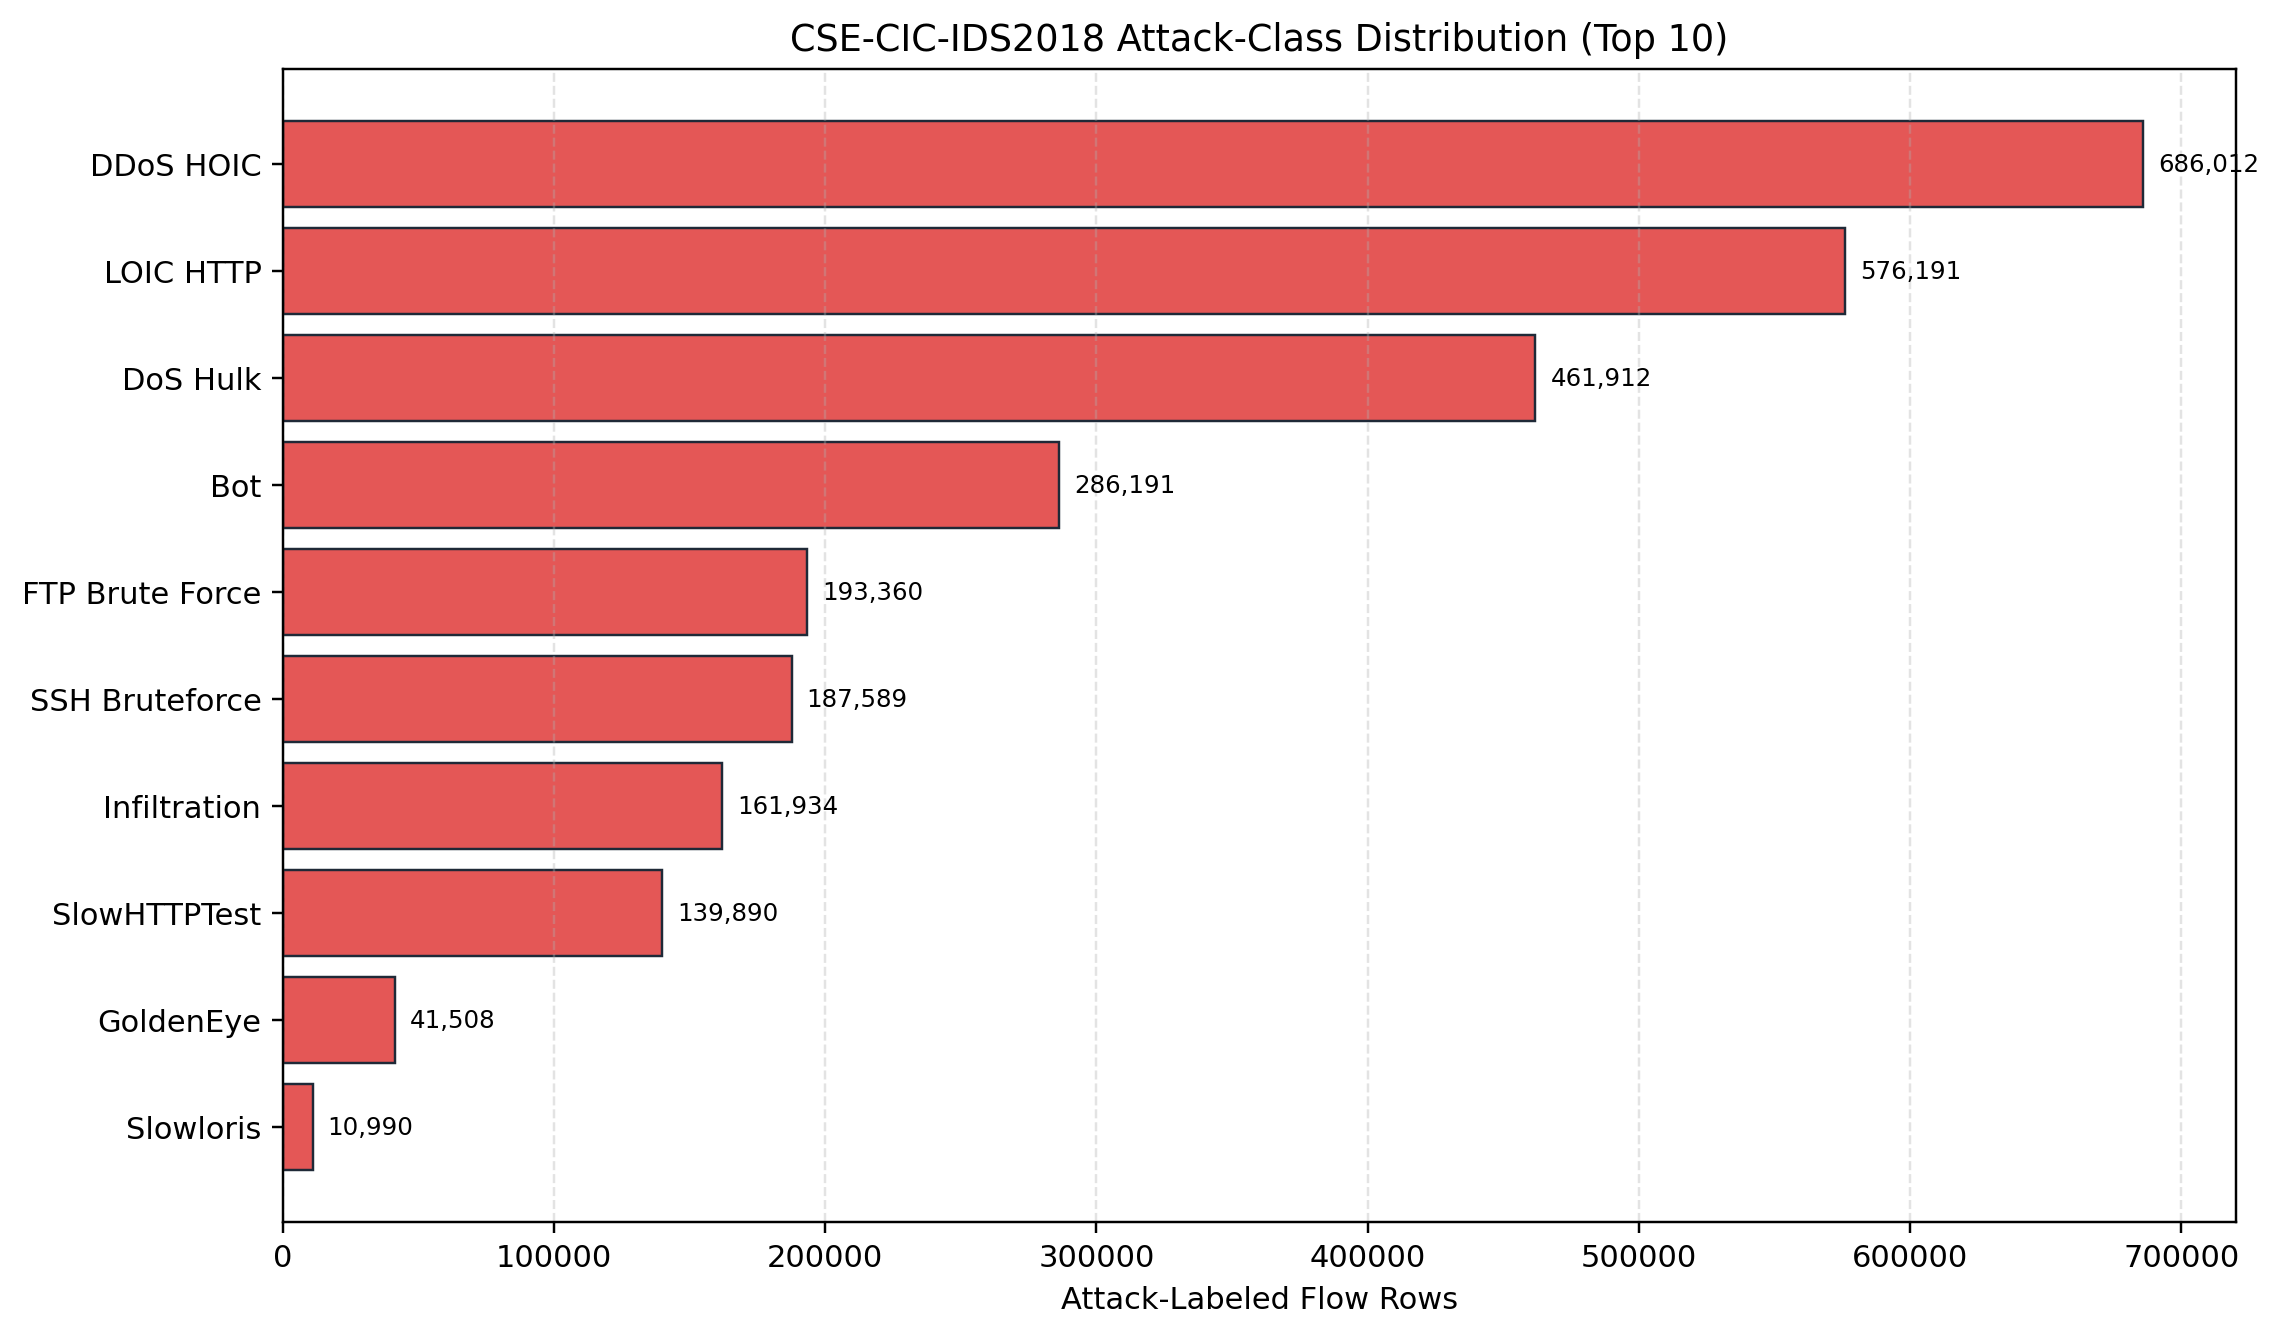
\includegraphics[width=\linewidth]{dataset_attack_distribution.png}
    \caption{Attack-class distribution in the retraining corpus, excluding the dominant benign class for readability.}
    \label{fig:dataset}
\end{figure}

Instead of inspecting single packets in isolation, traffic is grouped into two-way streams. Each stream is formed from the IPs at both ends, along with port numbers and protocol type. By examining these grouped exchanges, patterns in speed, sequence, balance, and combined traits become easier to identify. Packet totals appear alongside size distributions, bytes per second are measured, and timing between arrivals is recorded. Direction-based indicators emerge as well, along with summaries based on TCP flags, packet reuse patterns, TTL diversity, and header sizes. Unusual surges, irregular spacing, or strange signaling often reveal malicious behavior, especially when payload contents remain hidden. The features used here capture those subtle signs without needing to inspect deeper content.

One layer of the system relies on machine learning and is built around several models with distinct roles. The autoencoder measures reconstruction error to surface flows that do not resemble the learned normal baseline. Isolation Forest highlights flows that are easy to isolate as outliers, while K-Means measures deviation from learned cluster centers. Random Forest and gradient-boosted trees provide the strongest supervised classification layer for known attack categories. PPO and GNN models provide additional attack-likelihood signals that can be compared against the core models during scoring. Together, these models provide both anomaly awareness and labeled attack recognition.

These models work together rather than in isolation. Every output is logged by the system, which then forms an overall sense of risk based on current activity patterns. What makes this layered analysis valuable is that each model highlights different kinds of behavior. One model may treat traffic as normal, while another designed to detect anomalies may raise concern. Similarly, some flows may resemble known threats even if their anomaly scores remain low. Because the interface shows where models agree or disagree, it helps clarify the reasoning behind each alert. The operator can also choose which models are active from the Model Controls tab, making the platform useful for experimentation as well as monitoring.

A built-in rule-based mechanism adjusts alert severity when necessary. It exists because raw model predictions are sometimes too cautious under real traffic conditions. For example, repeated ping traffic, sudden bursts of connection attempts, suspicious packet-injection signatures, or intense UDP transmission may deserve attention even if they receive a low-risk label. These rules step in where the models hesitate and help connect automated scoring to practical operator review. While the models drive most decisions, exceptions based on recognizable patterns help guide urgency.

A major strength of the project is its support for active experimentation. Rather than relying only on fixed datasets, it produces dynamic attack patterns through Scapy. These trials include actions such as ping floods, SYN floods, UDP floods, and port scans. Every run records contextual details including attack type, destination address, target endpoints, packet volume, and start time. Each trial leaves behind structured logs for later inspection. When live traffic appears, the system attempts to match it against earlier test runs by comparing timing, destination, communication method, and channel information. As a result, the dashboard can show which flows matched, when they were detected, and how quickly protection started for individual tests.

The prevention layer is configurable by design. Operators can turn automatic blocking on or off and choose the severity level required before intervention occurs. Rather than depending on automation alone, users can manually block or unblock IP addresses, deploy decoy services, watch suspicious hosts without immediately containing them, or shield local ports that appear under targeted probing. Firewall actions rely on native operating system tools, such as \texttt{netsh advfirewall} on Windows. To prevent critical mistakes, safeguards exclude certain address types from being blocked, including loopback interfaces, multicast ranges, unspecified addresses, and local host entries. Blocked IP addresses and prevention settings are now saved across reboots and reliably appear on the dashboard after a refresh.

\section{Results}

The project now exists as a complete prototype rather than a collection of disconnected code files. Instead of isolated scripts, the system pulls live network data directly from the wire. From ingestion to analysis, traffic is converted into flow summaries on the fly. After transformation, machine learning models evaluate each flow with little noticeable delay. Results then appear on a visual interface almost immediately after processing. Metrics shown include flow counts, flagged events, blocked IPs, side-by-side model outputs, active blocking status, frequent communicators, suspicious exchanges, sensor health checks, decoy activity, and records from simulated intrusions. What once focused only on algorithm tuning now supports broader inquiry. This integration marks important progress because it enables testing, observation, and practical validation under realistic conditions. Figure~\ref{fig:dataset} highlights the breadth of the retraining corpus by showing the largest attack classes used in the current dataset refresh.

To improve robustness, the model stack was retrained on a much larger version of the CSE-CIC-IDS2018 dataset. The most recent full training run used 4,178,075 rows with 52 retained features. That larger-scale retraining refreshed the Random Forest, gradient-boosted tree, PPO, GNN, K-Means, autoencoder, and Isolation Forest artifacts that are now shipped with the project.

\begin{figure}[t]
    \centering
    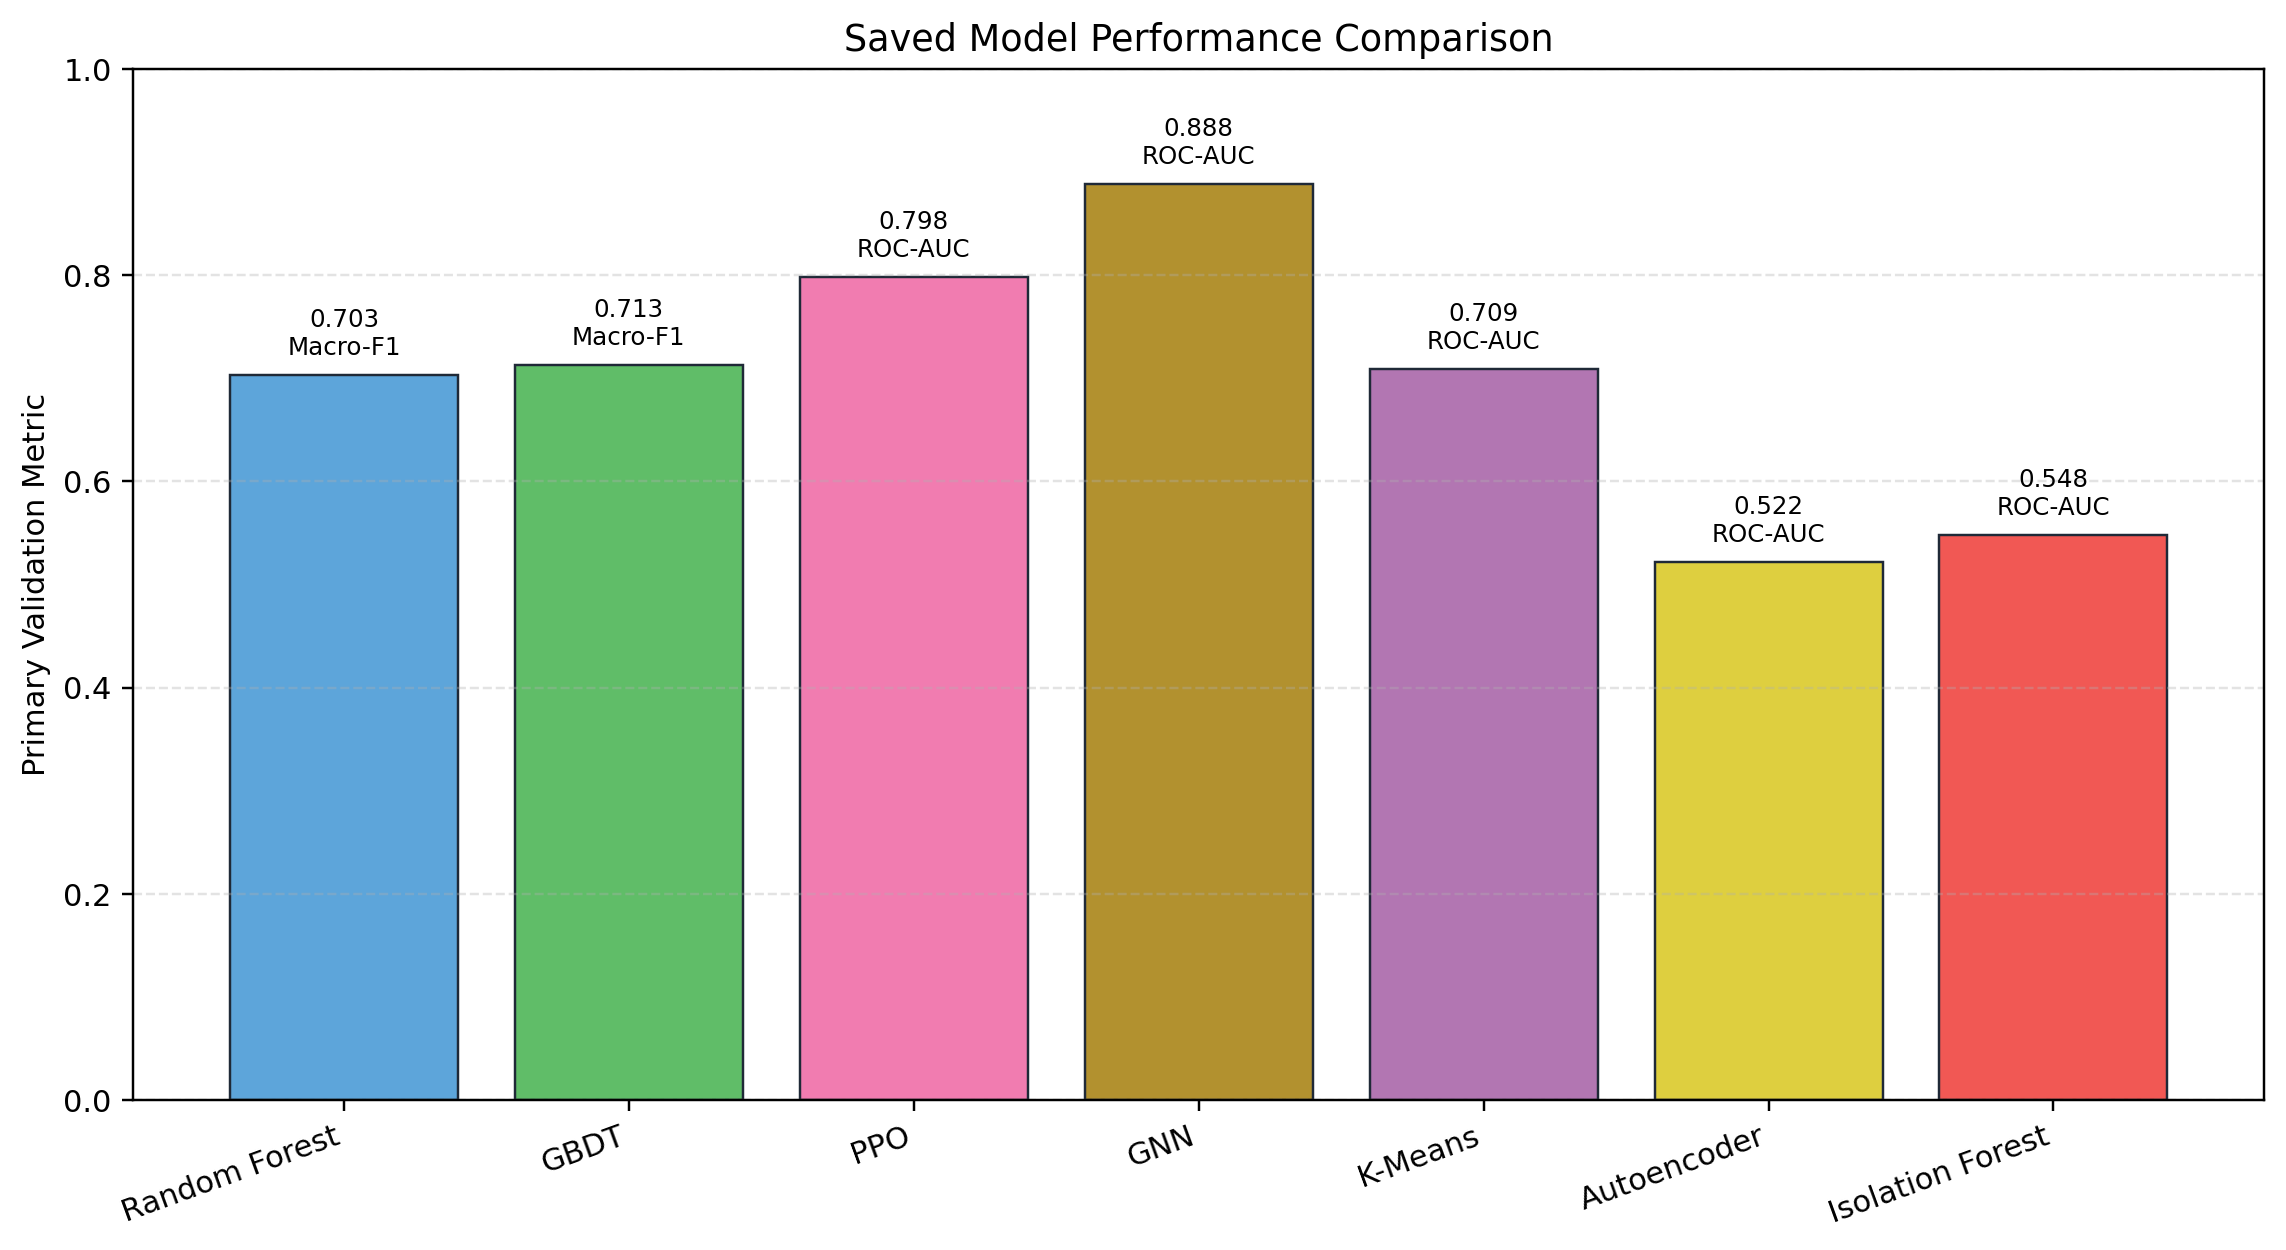
\includegraphics[width=\linewidth]{model_comparison_bar.png}
    \caption{Direct comparison of the saved model families using their primary validation metric. Supervised models are reported with macro-F1, while anomaly-oriented models use ROC-AUC.}
    \label{fig:modelbars}
\end{figure}

\begin{figure}[t]
    \centering
    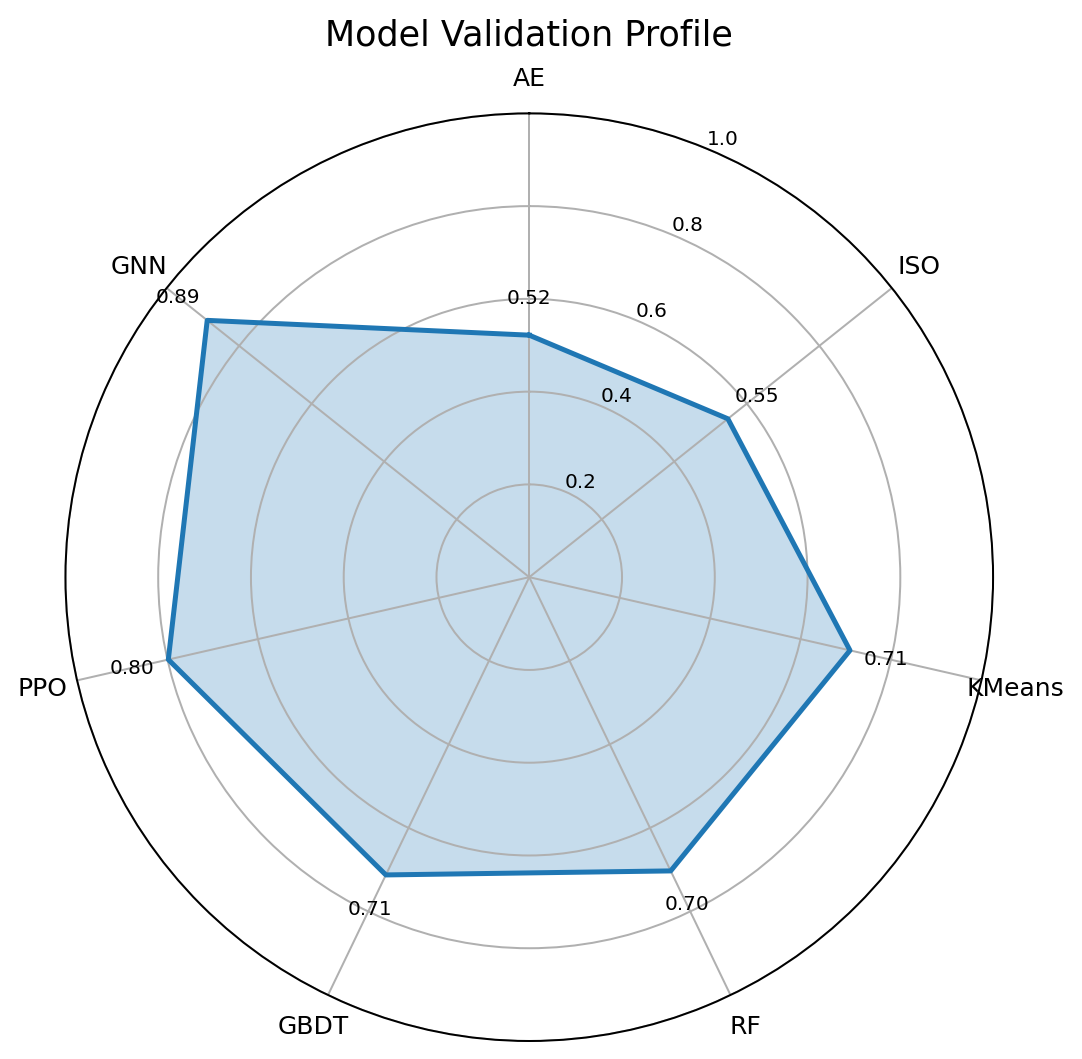
\includegraphics[width=\linewidth]{model_radar.png}
    \caption{Model validation profile from the current training report. Values reflect the primary saved validation metric for each model family, such as macro-F1 for supervised classifiers and ROC-AUC for anomaly-oriented models.}
    \label{fig:radar}
\end{figure}

Figures~\ref{fig:modelbars} and~\ref{fig:radar} summarize the current training profile. The strongest supervised results came from the retrained Random Forest and gradient-boosted tree models. Random Forest reached 85.0\% accuracy with a macro-F1 of 0.703, while the gradient-boosted tree reached 92.0\% accuracy with a macro-F1 of 0.713. PPO produced 84.3\% binary accuracy with ROC-AUC 0.798, and the GNN produced 88.0\% binary accuracy with ROC-AUC 0.888. Among the unsupervised models, K-Means remained the most useful with ROC-AUC 0.709, whereas the autoencoder and Isolation Forest reached ROC-AUC values of 0.522 and 0.548 respectively and therefore are now treated more cautiously in the live ensemble.

The replay system also became a useful benchmarking tool. It now supports curated attack-profile PCAPs, baseline PCAPs, and mixed traffic PCAPs, with separate reporting for attack detection and baseline quietness. In practice, that replay path is now used to compare how the tuned model stack behaves on controlled malicious samples versus quieter baseline captures without relying on screenshots or manual dashboard interpretation.

Testing in live conditions reveals both the strengths and limitations of the layered approach. One major benefit is that the system explains outcomes by model instead of producing only simple yes-or-no results. Because of this, users can trace suspicious alerts back to anomaly detectors, supervised classifiers, or rule-based triggers. Another advantage is the tracking of matched flows, first alert times, and first prevention times during simulated attacks. With these metrics logged, timing analysis becomes just as valuable as classification accuracy when judging system behavior.

At the same time, live testing revealed false positives. When the dashboard loads external resources over HTTPS, that traffic can sometimes be flagged as suspicious. As a result, a public IP may appear in the alert stream even when the intended test actually came from a private \texttt{10.x.x.x} host. This is important because it highlights how difficult it is to separate meaningful signals from background noise in behavior-based security systems. Since timing overlap between legitimate browser activity and test traffic can confuse model outputs, several improvements have already followed. These include better blocked-IP visibility, improved packet capture behavior on Windows, persistent state across sessions, tighter automatic blocking control, more careful alert deduplication, and stronger packet-level replay features for attack validation.

Operational safety has also improved. Earlier testing showed that turning protection off did not always remove old firewall blocks. After backend revisions, switching off automatic blocking now clears only system-generated rules while preserving blocks created manually by the operator. The defense layer is also no longer limited to simple IP blocking: watchlisting, inbound-only containment, port shielding, and adaptive decoy deployment provide multiple response strategies depending on operator goals.

Even with these improvements, the project is still better described as an advanced prototype than a completed study. Different software setups were used when building the machine learning components, which can still create compatibility issues if the environment drifts too far from the saved runtime assumptions. Stronger testing remains necessary as well, including repeated controlled trials, clearer evaluation metrics, and more structured reporting on precision, recall, false positive rates, false negative rates, and response times by attack type.

\section{Conclusion}

This work shows how stacking intrusion detection and prevention methods such as anomaly detection, supervised classification, real-time packet capture, simulated attacks, dynamic response, and decoy-based deception can produce a functioning prototype. Built around an autoencoder, Isolation Forest, K-Means clustering, Random Forest, gradient-boosted trees, PPO, and GNN components, the system observes network traffic, compares predictions side by side, generates warnings, and can enforce or stage multiple forms of response when needed. Through supervised testing in live conditions, it moves beyond standard coursework and becomes a platform suitable for both practical trials and deeper security research.

Although still evolving, the current version already provides useful capabilities. Capturing network traffic is one of its core functions, and analyzing flow behavior follows naturally from that. Live demonstrations run reliably, supported by integrated analysis tools. During tests, the system logs attack activity while also preserving blocked-IP state between restarts. At the same time, real-world complexity remains visible: models sometimes misclassify legitimate traffic, unrelated background activity interferes with experiments, and environment inconsistencies introduce technical issues. These outcomes matter not because they fit ideal theory, but because real deployments are messy in ways that controlled studies rarely capture.

Improving rigor and reproducibility should guide the next stage of development. First, model artifacts and runtime dependencies should be aligned to remove compatibility warnings and ensure stable operation. After that, testing should be strengthened through repeated runs under controlled conditions, using metrics such as precision, recall, false positives, false negatives, and detection delay by attack category. Another important step is reducing interference from irrelevant traffic, whether through filtering, emphasizing internal test flows, or removing unnecessary external dashboard dependencies. As these distractions are reduced, the system will become more stable and reliable. Only then can this promising early version mature into something robust enough for serious study.

\begin{thebibliography}{99}

\bibitem{denning87}
D. E. Denning, ``An Intrusion-Detection Model,'' \emph{IEEE Transactions on Software Engineering}, vol. SE-13, no. 2, pp. 222--232, Feb. 1987, doi: 10.1109/TSE.1987.232894.

\bibitem{roesch99}
M. Roesch, ``Snort - Lightweight Intrusion Detection for Networks,'' in \emph{Proceedings of the 13th USENIX Conference on System Administration (LISA XIII)}, Seattle, WA, USA, 1999, pp. 229--238.

\bibitem{paxson99}
V. Paxson, ``Bro: A system for detecting network intruders in real-time,'' \emph{Computer Networks}, vol. 31, nos. 23--24, pp. 2435--2463, Dec. 1999, doi: 10.1016/S1389-1286(99)00112-7.

\bibitem{lee00}
W. Lee and S. J. Stolfo, ``A framework for constructing features and models for intrusion detection systems,'' \emph{ACM Transactions on Information and System Security}, vol. 3, no. 4, pp. 227--261, Nov. 2000, doi: 10.1145/382912.382914.

\bibitem{patcha07}
A. Patcha and J.-M. Park, ``An overview of anomaly detection techniques: Existing solutions and latest technological trends,'' \emph{Computer Networks}, vol. 51, no. 12, pp. 3448--3470, 2007, doi: 10.1016/j.comnet.2007.02.001.

\bibitem{liao13}
H.-J. Liao, C.-H. R. Lin, Y.-C. Lin, and K.-Y. Tung, ``Intrusion detection system: A comprehensive review,'' \emph{Journal of Network and Computer Applications}, vol. 36, no. 1, pp. 16--24, 2013, doi: 10.1016/j.jnca.2012.09.004.

\bibitem{buczak16}
A. L. Buczak and E. Guven, ``A Survey of Data Mining and Machine Learning Methods for Cyber Security Intrusion Detection,'' \emph{IEEE Communications Surveys \& Tutorials}, vol. 18, no. 2, pp. 1153--1176, 2016, doi: 10.1109/COMST.2015.2494502.

\bibitem{sommer10}
R. Sommer and V. Paxson, ``Outside the Closed World: On Using Machine Learning for Network Intrusion Detection,'' in \emph{2010 IEEE Symposium on Security and Privacy}, Oakland, CA, USA, 2010, pp. 305--316, doi: 10.1109/SP.2010.25.

\bibitem{chandola09}
V. Chandola, A. Banerjee, and V. Kumar, ``Anomaly detection: A survey,'' \emph{ACM Computing Surveys}, vol. 41, no. 3, pp. 1--58, 2009, doi: 10.1145/1541880.1541882.

\bibitem{breiman01}
L. Breiman, ``Random Forests,'' \emph{Machine Learning}, vol. 45, no. 1, pp. 5--32, 2001, doi: 10.1023/A:1010933404324.

\bibitem{liu08}
F. T. Liu, K. M. Ting, and Z.-H. Zhou, ``Isolation Forest,'' in \emph{2008 Eighth IEEE International Conference on Data Mining}, Pisa, Italy, 2008, pp. 413--422, doi: 10.1109/ICDM.2008.17.

\bibitem{macqueen67}
J. MacQueen, ``Some Methods for Classification and Analysis of Multivariate Observations,'' in \emph{Proceedings of the Fifth Berkeley Symposium on Mathematical Statistics and Probability}, vol. 1, Berkeley, CA, USA, 1967, pp. 281--297.

\bibitem{mukkamala02}
S. Mukkamala, G. Janoski, and A. Sung, ``Intrusion detection using neural networks and support vector machines,'' in \emph{Proceedings of the 2002 International Joint Conference on Neural Networks}, Honolulu, HI, USA, 2002, pp. 1702--1707, doi: 10.1109/IJCNN.2002.1007774.

\bibitem{mirsky18}
Y. Mirsky, T. Doitshman, Y. Elovici, and A. Shabtai, ``Kitsune: An Ensemble of Autoencoders for Online Network Intrusion Detection,'' in \emph{Proceedings 2018 Network and Distributed System Security Symposium}, San Diego, CA, USA, 2018, doi: 10.14722/NDSS.2018.23204.

\bibitem{shone18}
N. Shone, T. N. Ngoc, V. D. Phai, and Q. Shi, ``A Deep Learning Approach to Network Intrusion Detection,'' \emph{IEEE Transactions on Emerging Topics in Computational Intelligence}, vol. 2, no. 1, pp. 41--50, 2018, doi: 10.1109/TETCI.2017.2772792.

\bibitem{tavallaee09}
M. Tavallaee, E. Bagheri, W. Lu, and A. A. Ghorbani, ``A detailed analysis of the KDD CUP 99 data set,'' in \emph{2009 IEEE Symposium on Computational Intelligence for Security and Defense Applications}, 2009, pp. 1--6, doi: 10.1109/CISDA.2009.5356528.

\bibitem{moustafa15}
N. Moustafa and J. Slay, ``UNSW-NB15: A comprehensive data set for network intrusion detection systems (UNSW-NB15 network data set),'' in \emph{2015 Military Communications and Information Systems Conference (MilCIS)}, 2015, pp. 1--6, doi: 10.1109/MilCIS.2015.7348942.

\bibitem{hinton06}
G. E. Hinton and R. R. Salakhutdinov, ``Reducing the Dimensionality of Data with Neural Networks,'' \emph{Science}, vol. 313, no. 5786, pp. 504--507, 2006, doi: 10.1126/science.1127647.

\end{thebibliography}

\end{document}
